\vspace*{\fill}

\noindent\hrulefill\quad\raisebox{-0.24em}{\scshape\normalsize \textbf{Abstract}}\quad\hrulefill

\bigskip

Real-time strategy (RTS) games are among the most demanding benchmarks for sequential decision-making: players gather resources, coordinate many units, and plan over long horizons, in real time and within a combinatorial action space. AlphaStar reached Grandmaster level in StarCraft~II, but at the cost of hundreds of accelerators running for weeks, beyond academic reach. MicroRTS distills these difficulties onto small grid maps while keeping training tractable on a modest budget, making it the reference academic testbed and the subject of an annual competition since $2017$.

\medskip

This master's thesis investigates deep reinforcement learning (DRL) for MicroRTS, guided by two questions: \emph{which architectural and algorithmic design decisions most improve a MicroRTS agent}, and \emph{whether one competitive with the strongest prior competition entries can be trained within an academic compute budget}. Taking RAISocketAI, the first DRL agent to win the competition, as reference and starting from the Gym-$\mu$RTS GridNet baseline, every design decision is evaluated in isolation before combining the best ones. The work contributes \textbf{\emph{(i)}}~a reproducible Conference on Games (CoG)-style tournament framework over twelve maps and fifteen reference agents under five ranking metrics; \textbf{\emph{(ii)}}~an extended, modular Java--Python environment stack with composable wrappers and vectorized self-play; \textbf{\emph{(iii)}}~the \code{UECD} architecture, fusing multi-scale convolution, entity-level Transformer reasoning, and bottleneck self-attention to cover an RTS network's local, relational, and global demands; \textbf{\emph{(iv)}}~a modular PPO pipeline whose mechanisms are ablated individually; and \textbf{\emph{(v)}}~a formal analysis of a discount-induced reward collapse under shaped-to-sparse annealing.

\medskip

The resulting agent, \code{UECD-Best}, combines these under a two-phase opponent-curriculum fine-tuning schedule. On the \emph{basesWorkers16x16A} map, it tops a $19$-agent round-robin tournament ($96.67$\% win rate, first on four of the five metrics) and wins $65.7$\% of its head-to-head games against RAISocketAI, using $9.47$ GPU-days and ${\sim}350$\,M steps, below the ${\sim}23.6$ GPU-days and ${\sim}500$\,M steps RAISocketAI reports for its small-map subset. A second agent, \code{UECD-MultiMap}, trained across five layouts of three different sizes, spreads its competence evenly with no per-map collapse, showing that the padded environment and a prioritized-level-replay curriculum make cross-layout training feasible, though it does not yet match the single-map specialist's peak.

\bigskip

The open-source pipeline released with this thesis offers a DRL substrate for future generalist agents and hybrid DRL/LLM systems, as the competition shifts toward language-model-based agents.

\bigskip

\begin{center}
\newcommand{\kwsep}{\;\textcolor{black!55}{\small$\bullet$}\;}
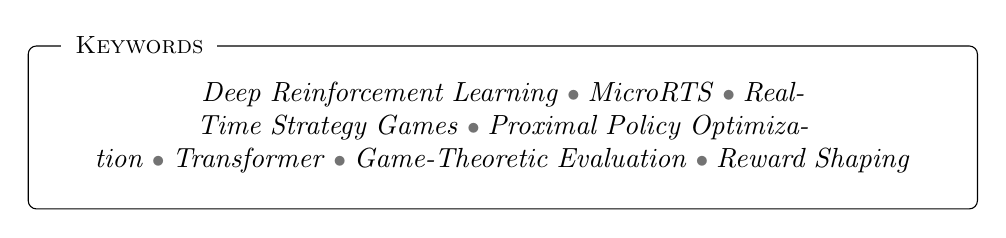
\begin{tikzpicture}
\node[draw=black, rounded corners=3pt, line width=0.4pt,
      inner xsep=14pt, inner ysep=13pt,
      text width=\dimexpr\linewidth-30pt\relax, align=center] (kwbox)
  {\emph{Deep Reinforcement Learning}\kwsep\emph{MicroRTS}\kwsep%
   \emph{Real-Time Strategy Games}\kwsep\emph{Proximal Policy Optimization}\kwsep%
   \emph{Transformer}\kwsep\emph{Game-Theoretic Evaluation}\kwsep\emph{Reward Shaping}};
\node[anchor=west, fill=white, inner xsep=5pt]
      at ([xshift=12pt]kwbox.north west) {\scshape\small Keywords};
\end{tikzpicture}
\end{center}

\vspace*{\fill}